\documentclass{kybernetika}
%the class kybernetika includes these packages:
% graphicx, amssymb, amsmath

%--------------------------------------------------------------------------------------------------
% used environment for theorems:

\newtheorem{theorem}{Theorem}[section]
\newtheorem{lemma}[theorem]{Lemma}
\newtheorem{proposition}[theorem]{Proposition}
\newtheorem{corollary}[theorem]{Corollary}
\newtheorem{remark}[theorem]{Remark}
\newtheorem{fact}[theorem]{Fact}
\newtheorem{example}[theorem]{Example}
\newtheorem{definition}[theorem]{Definition}
\newtheorem{observation}[theorem]{Observation}

\begin{document}

%==================================================================================================
% TITLE PAGE 
%==================================================================================================
\pagestyle{myheadings}
\title{Application of Long Short Term Memory neural networks for GPS satellite clock 
bias prediction}

\author{Piotr Gny\'{s}, Pawe\l{} Przestrzelski}

\contact{Piotr}{Gny\'{s}}
{Department of Computer Science,  Polish-Japanese Academy of Information Technology,
Koszykowa 86 Street, 02-008 Warsaw}{pgnys@pjwstk.edu.pl}

\contact{Pawe\l{}}{Przestrzelski}
{Department of Computer Science,  Polish-Japanese Academy of Information Technology,
Koszykowa 86 Street, 02-008 Warsaw}{pprzestrzelski@pjwstk.edu.pl}

\markboth{Piotr Gny\'{s}, Pawe\l{} Przestrzelski}{LSTM networks for GPS clock bias prediction}

\maketitle

\begin{abstract}
In this article the results of an application of Long Short Term Memory neural networks for
clock bias will be presented and compared against current state of the art in real-time
GPS clock bias prediction. Presented approach is intended to better quality of localization
for marine robots that operate autonomously for long periods of time away from convenient  
internet uplink.
\end{abstract}

\keywords{LSTM, Long Short Term Memory, Neural Networks, GPS, Navigation, Time series prediction}

\classification{68T05, 68T10, 68T40}


%==================================================================================================
\section{Introduction}
Research presented in this paper is part of a larger project that aims at developing a long
term autonomous marine robotics systems. However as Global Positioning System (GPS) is used
in many application elements specific to one that was intended when working on algorithm will
be omitted with exception of MOTIVATIONS section.

%--------------------------------------------------------------------------------------------------
\subsection{Motivation}
In recent years there was a rise in popularity of autonomous platforms. Examples include, but
are not limited to, Tesla self driving cars, autonomous container ships or robotic defence 
systems. All those applications have one thing in common, they require a precise navigation 
capabilities that will allow them to move without damaging themselves or their environments. 
This is especially challenging in marine environment as not only there is almost no visual
reference points on open see but also because any contact with external data source is expensive
as very often only connection available is satellite uplink.
In case of large vessels, like already mentioned autonomous container ships, this is only
problem of bandwidth cost. 
However in case of small robots like gliders or sailboats that rely on low power consumption 
any localization system is limited by low computation power and high energy consumption of 
satellite communication that discourages it frequent use.
This is why an effort was made to deploy a solution that provides a on-board solution for high
quality GPS based localisation with low computational overhead.

%--------------------------------------------------------------------------------------------------
\subsection{Contribution}
In following paper a new approach for GPS clock bias prediction based on a Long Short Term Memory
neural networks is presented. For 20 out of 29 satellites that were analysed in this work 
prediction results were better than current state of the art and for 6 of them results were
significantly better. Results of presented research can be used in a offline GPS receiver as 
a alternative for IGU provided products.


%==================================================================================================
\section{Clock bias in GNSS}
Due to the nature of GNSS precision time measurement is crucial for correct localisation.
In this section more inforation about why it is so and what is current state of the art on this
topic will be presented.

%---------------------------------------------------------------------------------------------------
\subsection{Importance of clock bias in localisation}
All global satellite navigation systems (GNSS) are variant of beacon based localization
systems\cite{Blewitt1997}.Such systems require information about beacon position
and distance between localized object and beacons.
With that information it is possible to calculate position of object in same reference
frame as that of beacons.
Both of those tasks are much more difficult in GNSS due to a nature of the beacons.
Unlike in case of a stationary beacons GNSS satellites move with high speed so
their position must be calculated based on satellite ephemeris\cite{Vallado2008}.
Another problem is distance measurement which without specialised equipment must be
done with time of arrival (ToA) instead of angle of arrival (AoA) or
received signal strength (RSS) \cite{Doberstein2012}.
When measuring distance by ToA  3 properties of a signal must be known:
\begin{itemize}
\item $t_o$ : time of origination
\item $t_a$ time of arrival
\item $v$ velocity
\end{itemize}
In case of GNSS system signal is a electromagnetic wave therefore its speed is equal
to speed of light $c\approx 3*10^{9} \frac{m}{s}$. Time of arrival is recoded when
data frame wavefront reaches receiver, this means that receiver time is used.
Origination time is recorded on satellite according to it local clock and
included in data frame. Thanks to that distance can be calculated by simple
equation:
\begin{equation}
  d=c*(t_a-t_o)
\end{equation}
However $t_a$ and $t_o$ are using different reference frame so for comparison
to be possible they must be transformed into a common reference frame.
This is refered to as a synchronisation of the clocks and is very important as
a desynchronisation on level of single nanosecond results in about 30 cm of
positioning error\cite{Enge2011}.
While actual calculations 

%--------------------------------------------------------------------------------------------------
\subsection{IGU products}
The most widely used source of precise clock corrections are products provided 
by International GNSS Service (IGS) \cite{IGS}.
% TODO:Fix table size so it is not wider than text
\begin{table}[ht] 
	\centering
	\caption{Variants of IGS products}
	\label{tab:igs_products}
	\begin{tabular*}{\textwidth}{*{5}{l}}
		\hline
		\hline
		Type& Accuracy& Latency& Update& Sample \\
		&&&&interval\\
		\hline
		Transmitted & 5ns & real time & -- & daily  \\
		Ultra rapid -- predicted & 3ns & real time & at 03, 09, 15, 21 UTC & 15 min  \\
		Ultra rapid -- observed & 150ps & 3-9 hours & at 03, 09, 15, 21 UTC & 15 min  \\
		Rapid & 75ps & 17-41 hours & at 17 UTC daily & 5 min \\
		Final & 75ps & 12-18 days & every Thursday & 30 s \\
		\hline
		\hline
	\end{tabular*}
\end{table}
Values shown in Table \ref{tab:igs_products} refer to satellite clock bias only,  IGS products
provide other information which full description  is available at online repositiory. 
IGS products can be easily divided into two categories:
\begin{itemize}
	\item real time consisting of transmitted and ultra rapid predicted half,
	\item high latency consisting of ultra rapid observed half as well as rapid and final products.
\end{itemize}
Solutions that have high latency are not usable in real-time navigation and as such will not be
considered in this work. Ultra-rapid observed part will be used as a source of
reference time so that if a bias prediction error is equal to zero it means that is
the same as provided by Ultra-rapid observed.
As can be seen in the Table \ref{tab:igs_products} all real-time solutions provide precision 
at a range of nanoseconds, aim of this work is to show that LSTM networks can provide 
better results than those solutions while still working at real-time response latency.

%--------------------------------------------------------------------------------------------------
\subsection{Data source}
This work focuses only on GPS satellites which are divided into five groups :
Original (II), IIA, ,IIR ,IIR-M ,IIF.
As original generation was full retired in 2007 it will not be taken into consideration, while
a single satellite from generation IIA was used in second phase of experiments it was no longer
presend in following phases as that generation was fully retired in 2019.
This results in 31 individual satellites for phases 1 and 2 and 30 for phases 3 and 4.
Almost all of them are equipped with Rubidium clock ensemble witch exception of two satellites
from generation IIF that use Cesium clocks instead.
Each satellite have an assigned space vechicle number (SVN) and pseudo random noise (PRN).
In this work a PRN will be used as a identifier as it is unique for every active satellite, 
although it can be used again after said satellite gets retired, and ranges from 1 to 32.
\begin{table}[ht] \label{table:2}
\parindent0pt
\caption{Bias prediction error in relation to regularization and dropout level}
\centering
\begin{tabular}{ l  c  c }
  \hline
  \hline
  Generation& clock typt& satellites\\  \hline
  IIA & Rb& 18\\  
  IIR & Rb& 2 11 13 14 16 19 20 21 22 23 28\\ 
  IIR-M & Rb& 5 7 12 15 17 29\\ 
  IIF & Rb& 1 3 6 9 10 25 26 27 30 32\\ 
  IIF & Cs& 8 24 \\ \hline \hline
 \end{tabular}
\end{table}
For satellites with rubidium based clock ensembles bias have a very disting constant drift
that makes data appear linear, it can be seen for satellites 01 and 08. 
On the other hand in case of cesium based clock ensembles for which constant drift is much 
smaller other sources of bias are visible, like seen for satellite 24.
There is also a single satellite for which, during observed period, constant drift was almost
not present. This was satellite 14 and while no official source of information describes this 
behaviour
\begin{figure}[ht] 
\centering
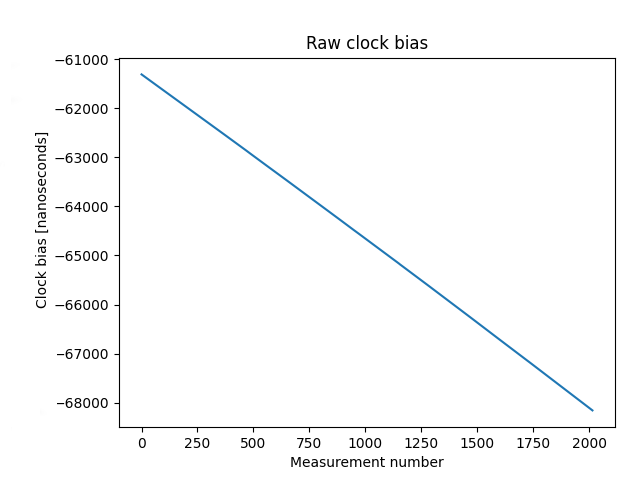
\includegraphics[width=10cm]{res/bias_raw.png}
\caption{Raw clock bias}
\label{fig:bias_raw}
\end{figure}

\end{document}


